\chapter{Guidelines and Desiderata for Optimizing the Physical Data Layout and Query Processor in GDBMSs}
\label{c:guidelines}

In this chapter, we review the components of storage layer, primary query plan operators, and the general data access patterns of operators when evaluating a query in a \gls{gdbms}. We then draw a basic set of guidelines and desiderata that will instruct the physical data layout of our columnar data structures and query-processing techniques introduced in later chapters.

Section \ref{sec:property-graph-data-model} briefly describes the \emph{property graph data model}. Section \ref{sec:storage-components} describes the primary storage components of \gls{gdbms}s that adopt the property graph data model, while Section \ref{sec:operators} reviews the query processing operators in \gls{gdbms}s. We end the chapter by stating our guidelines in Section \ref{sec:guidelines}.

\section{Property Graph Data Model}
\label{sec:property-graph-data-model}

\begin{figure}
	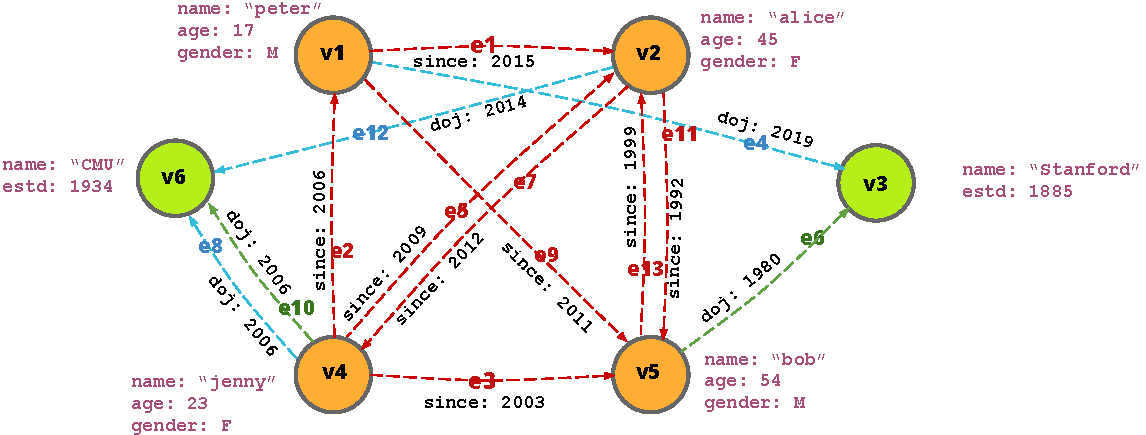
\includegraphics[scale=0.86]{img/property-graph}
	\vspace{-8pt}
	\caption{Running example graph.}
	\label{fig:runn}
	\vspace{-8pt}
\end{figure}

Figure~\ref{fig:runn} shows a graph data represented using the property graph data model, that will serve as our running example in this thesis. A property graph consists of \emph{vertices}, that represent entities, and directed \emph{edges} between vertices, that represent relationships between entities. Each vertex and edge has a particular \emph{label}, describing the high-level categories of vertices and edges. For example, in Figure~\ref{fig:runn}, vertices have labels: \texttt{PERSON} and \texttt{ORG}, while edges have labels: \texttt{FOLLOWS}, \texttt{WORKAT}, and \texttt{STUDYAT}.

Similar to columns in relational tables, vertices and edges can have key-value \emph{properties}. Although the properties of vertices and edges do not need to adhere to a strict \emph{schema}, in practice many of these properties are often highly structured, i.e., the same set of properties exists on all the vertices and edges of the same vertex and edge label respectively.

\section{Primary Storage Components in GDBMSs}
\label{sec:storage-components}

In every \gls{gdbms} we are aware of, the edges of a graph are stored in an data structure called \emph{adjacency lists}~\cite{bonifati-adj-lists}. An adjacency list of a vertex $v$ is a list of $v$'s \emph{adjacent} edges and the corresponding  \emph{neighbouring} vertices. Each vertex has 2 adjacency lists: a \emph{forward adjacency list} containing all outward edges of that vertex, and a \emph{backward adjacency list} that holds all inward edges of the vertex. One can think of edges in the graph as a relational table with 3 attributes: a source vertex, a destination vertex, and an 8-byte edge ID. The adjacency lists can then be thought of as an \emph{index} on this relational table that is \emph{clustered} by either the source or destination vertex. In practice, this indexing structure often has a depth of 1 or 2, hence, given the ID of a vertex $v$, a system can access $v$'s list of adjacent edges and neighbour vertices in 1 or 2 lookups. By having adjacency lists of a vertex in either direction, the system can access the list of outward and inward edges as well as the neighbouring vertices of a vertex in a constant-time lookup operation, which provides the core capability of fast joins on vertices to a \gls{gdbms}. 

Typically, the adjacency list of a vertex is further clustered into sublists grouped by the edge label. This enables traversing the neighbourhood of a vertex based on a \emph{particular} label in constant time. The rationale behind the sub-clustering is that queries made by applications often have specific labels on query edges. Some systems further order the edges in the adjacency lists either by a specific property associated with the adjacent edges or neighbour vertices, such as \emph{location} or \emph{timestamp}, or simply by neighbour vertices' IDs. Sorting enables the system to access parts of lists in time logarithmic in the size of the adjacency list.

A \gls{gdbms} also stores properties associated with the vertices and the edges. A straightforward approach is to store properties in a \emph{key-value store} \cite{dgraph} and use the property key and the vertex or edge ID as the key into the store. Properties can also be stored in an \emph{interpreted attribute layout} \cite{beckmann:sparse}, where a record of a vertex or an edge consists of the the key-value pairs of that particular vertex or edge, and is variable-sized depending on the size of keys and values data. However, searching for a property in variable-sized records involves decoding and parsing the entire record until the matching attribute is found, which can be expensive. Another way of storing properties is using doubly linked-lists, as done in Neo4j \cite{neo4j}, where the system keeps track of a pointer to the first property record of a vertex or edge and each subsequent property record stores a pointer to the next property record. This is a cache-inefficient layout since it does not organize the properties of vertices and edges in the order in which they would be accessed in query execution. 

\section{Query Execution in GDBMSs}
\label{sec:operators}

In this section, we review the general query execution in a \gls{gdbms} by analyzing the major operators used in query plans. Although systems differ in their architectures and implementation of operators that they support for executing queries, they still exhibit similarities in their data access patterns. We use the Cypher query language \cite{cypher} to describe the queries we use in our examples. A user query typically consists of 3 parts: 1) a \texttt{MATCH} clause that describes a subgraph query pattern $Q(V_Q, E_Q)$, where $V_Q$ and $E_Q$ are the query vertex and edge variables, respectively, that the system will match on the input graph; 2) a \texttt{WHERE} clause the contains a predicate $\rho$ over properties of the edges and vertices that the matched subgraph must satisfy; and 3) a \texttt{RETURN} statement that returns a projection of the variables in the match query or performs a group-by and aggregate information. The \texttt{MATCH}, \texttt{WHERE}, and \texttt{RETURN} clauses of a Cypher query effectively corresponds to the \texttt{FROM}, \texttt{WHERE}, and \texttt{SELECT} clauses of SQL. Example \ref{ex:cypher-example} shows a typical query written in Cypher, that queries the example graph in Figure~\ref{fig:runn}.

\begin{example}
	\vspace{5pt}
	\label{ex:cypher-example}
	Example Cypher query. 
	{\em 
		\begin{lstlisting}[numbers=none,  showstringspaces=false,belowskip=0pt ]
		MATCH (a:PERSON)$-$[e:WORKAT]$\rightarrow$(b:ORG)
		WHERE a.age $>$ 22 AND b.estd < 2015
		RETURN *\end{lstlisting}
	}
	\noindent This query returns all \texttt{PERSON} vertices and their workplaces, constrained by the condition that the \textsc{\char13}\texttt{age}\textsc{\char13} property of all \texttt{PERSON} vertices has a value greater than 22 and the \textsc{\char13}\texttt{established}\textsc{\char13} property of all \texttt{ORG} vertices is less than 2015. $a$ and $b$ are query vertex variables while $e$ is a query edge variable.
\end{example}

The following are the major operators used for matching a subgraph pattern and evaluating predicates in a query.

\begin{itemize}
	
	\item \textbf{\texttt{SCAN}}: Scans a set of vertices and edges from the graph topology.
	
	\item \textbf{\texttt{NEIGHBOURHOOD JOIN}} (e.g. \texttt{EXTEND/INTERSECT} in Graphflow; \texttt{EXPAND} in Neo4j): At a high level, the join operator matches the subgraph query pattern $Q$, one edge at a time. Some systems, e.g Graphflow, can also match cyclic queries by matching multiple edges at a time. The input to the operator is a partial match, $t$, that has already matched $k$ of the query edges in $Q$. For each partially match $t$, the operator extends $t$ by matching an unmatched query edge $e_q(u_q, v_q)$, where one of $v_q$ or $u_q$ has already been matched in $t$. Say $v_q$ has already been matched. The \emph{join} happens by sequentially reading adjacent edges and neighbour vertices one at a time from the forward or backward adjacency list of the matched $v_q$, to produce a $k+1$-match. The output of the \texttt{JOIN} is $t$ with newly matched $e_q$ and $u_q$.
	
	\item \textbf{\texttt{PROPERTY READER}}: The vertex or edge property reader reads a property value of any vertex or edge that has been assigned to a variable in $V_Q$ or $E_Q$ of a partial match $t$, from the underlying property storage. 
	
	\item \textbf{\texttt{FILTER}}: Given the predicate $\rho$ from the \texttt{WHERE} clause and a partial match $t$ of $Q$, the \texttt{FILTER} operator omits $t$ from the result of the query if $t$ does not pass predicate $\rho$.
	
\end{itemize}

\begin{figure}
	\hfill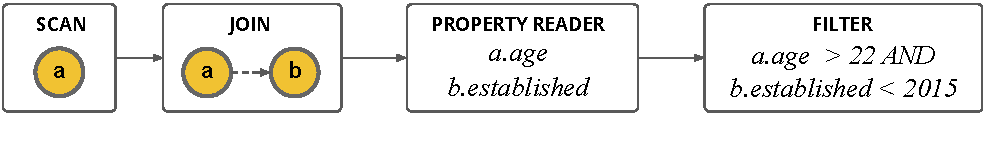
\includegraphics[scale=0.78]{img/ex-qp}\hfill
	\vspace{-10pt}
	\caption{Query plan for Example~\ref{ex:cypher-example}.}
	\vspace{-8pt}
	\label{fig:ex-qp}
\end{figure}

Figure~\ref{fig:ex-qp} shows one of the query plans that the system will generate to execute query in Example~\ref{ex:cypher-example}. It consists of the following sequence of operators: 1) \texttt{SCAN} operator that matches the variable $a$ in query to vertex in the graph having label \texttt{PERSON}; 2) \texttt{PROPERTY READER} reads the property \texttt{age} of the vertex matched to $a$; 3) \texttt{FILTER} operator filter out the partial match based on the constraint $a.age>22$; 4) \texttt{JOIN} operator matches $b$ by reading an adjacent edge and neighbour vertex from the forward adjacency list of $a$'s match; 5) \texttt{PROPERTY READER} reads the property \texttt{estd} of $b$'s match; and finally 4) another \texttt{FILTER} operator filters out the matched query pattern that do not confirm to the constraint $b.estd < 2015$.

\section{Guidelines and Desiderata}
\label{sec:guidelines}

We next outline a set of guidelines and desiderata for designing the physical data layout and query processor of a \gls{gdbms}.

\begin{guideline}[Edges are doubly-indexed.]
	\vspace{-5pt}
	Each edge appears in the forward adjacency list of that edge's source vertex and the backward adjacency list of its destination vertex. This results in a 2x replication factor in storing the topology of a graph in the system. This replication cannot be avoided by dropping an adjacency list in any one direction without hampering the capability to perform fast neighbour joins, which is one of the core features of a \gls{gdbms}. Therefore, we will also doubly index the edges in our design.
\end{guideline}


\begin{guideline}[Edge properties are read in the same order as edges in an adjacency list.]
	\label{ssec:edges-ordered}
	During the execution of a query, the \texttt{JOIN} operator will access the edges of a vertex $v$ in the order these edges appear in $v$'s forward or backward adjacency lists. If the query also needs to access the properties of these edges, the access to these edge properties will also be in the same order in which edges were read from the adjacency list. Given that the edges and edge properties are read in order, we define our first desideratum for the physical data layout and query processor:
	
	\begin{desideratum}
		\label{des1}
		Store the properties of edges in the order in which edges are ordered in the adjacency lists and read the edges and their properties sequentially in the operators.
	\end{desideratum}
	
\end{guideline}

\begin{guideline}[Vertices cannot be ordered to make access from all neighbour vertices sequential.]
	\label{gdln:vertices-unordered}
	Contrary to how the edges and edge properties can be strictly ordered for each of the adjacency lists, in general, there cannot be ordering on the vertices that completely localizes the access to neighbour vertices of every vertex and the properties of these neighbour vertices without prohibitive data replication. In general, if a vertex $v$ has $n$ neighbours, then $v$ and its properties need to be replicated $n$ times for localized access. Hence, localizing access to neighbour vertices and their properties should not be put in the desiderata of the system's physical data layout design. 	
\end{guideline}

\begin{guideline}[Access to vertex properties are random and many adjacency lists are very small.]
\label{gdln:fast-decompress}
Guideline~\ref{gdln:vertices-unordered} implies that the system should take it for granted that access to the vertex properties will require random accesses and will not be sequential. For example, when joining a node $v$ with its neighbours and accessing the \texttt{age} property of each neighbour, the accesses will be to non-consecutive locations in the vertex properties' storage based on the neighbour vertex IDs. Another property of real-world graphs is that adjacency lists of many vertices are very small because of the power-law distribution of adjacency lists. Systems should expect many very short adjacency lists, with only a few edges in them. Therefore during query processing with two or more joins, reading different adjacency lists and properties of these edges will require reading a short list followed by a random access and then reading another short list, and so on.

In an in-memory setting, which we focus on in this work, our aim with compression is not to achieve high compression ratios but to optimize for high decompression rates or to avoid decompression of data altogether, as compression schemes with slow decompression hurt performance. Moreover, techniques that require decompressing blocks of data, say a few KBs, to only read a single property or a single short adjacency list can be prohibitively expensive. Hence, our second desideratum is:
%We designed our columnar data structures for in-memory \gls{gdbms}. For these data structures, the focus with compression is not on achieving high compression ratios but to optimize for high decompression rates or to avoid decompression of data at all.
\begin{desideratum}
\label{des:compression}
If compression is used, the system should be able to decompress arbitrary single elements in a compressed block in constant time with respect to the block size.
\end{desideratum}  

\end{guideline}

\begin{guideline}[Graph data often has partial structure.]
	\label{gdln:graph-schema}
	Even though the property graph data model is semi-structured, in practice, graph databases stored in \gls{gdbms}s often have a structure in the data, which \gls{gdbms}s can exploit. One reason this structure exists is that, as observed in prior work \cite{survey}, the data in \gls{gdbms} often comes from structured data stored in \gls{rdbms}. In fact, several of the \gls{gdbms}s from industry and some academics are actively working on defining a schema language for the property graph data model \cite{schema-validation-bonifati, defining-schema-hartig}. We identify three commonly appearing structure in property graph data:
	
	\begin{enumerate}
		
		\item \textbf{Edge label determines the source and destination vertex labels.} Often, edge labels in the graph data have a well-defined set of source and destination vertex label(s). This restricts the vertices to having inward or outward edges of only a definite set of labels. In our example graph, edges with label \texttt{FOLLOWS} only exists between vertices of label \texttt{PERSON}.
		
		\item \textbf{Edge label has fixed cardinality.} The number of edges of a particular label to which a source or destination vertex can be associated is a property of the edge label. We call this the \emph{cardinality} of an edge label, similar to the cardinality of relationships in relational data. \emph{One-to-one} (1-1) cardinality for a label $l_e$ means that each source vertex can be connected to at most one destination vertex through an edge with label $l_e$ and vice versa. \emph{Many-to-one} (n-1) permits a single edge of a label from a source vertex but multiple edges to a destination vertex. Similar analogy can be applied to \emph{one-to-many} (1-n) and \emph{many-to-many} (n-n) cardinality edge labels.
		
		\item \textbf{Label determines properties on vertices and edges.} Similar to the attributes of a relational table, properties on an edge or vertex and the datatypes of these properties can \emph{often} be determined by its edge or vertex label. In our example graph, all vertices having the label \texttt{PERSON} have 3 properties: \texttt{name:STRING}, \texttt{age:INT} and \texttt{gender:STRING}. As long as a significant fraction of vertices and edges with a particular label have a common set of properties, a system can exploit this structured to store these properties more efficiently. 
		
	\end{enumerate}
	
	Such structure in data provides an opportunity to design more efficient and simpler data structures for accessing the storage layer of \gls{gdbms}. Our third desideratum is:
	
	\begin{desideratum}
		Exploit the above three commonly appearing structures in the graph data to (i) compress the data to save space; and (ii) provide faster access to the data.
	\end{desideratum}
	
	\vspace{-10pt}
	However, not all data in graph databases have well-defined structure. As a working terminology, we will use the following terms:
	
	\begin{itemize}
		\item \textbf{Structured and unstructured edge:} An edge of a particular label that follows above-mentioned points is called an structured edge. An edge that is not structured, is called an unstructured edge.
		
		\item \textbf{Structured and unstructured property:} A structured property is a property on a vertex or edge that; (i) can be determined by the label of that vertex or edge; and (ii) have the same data type in all its occurrence. We will also require that the property is not too sparse, i.e., appears in a significant fraction of the vertices of edges of a particular label. Any property that is not a structured property, is considered an unstructured property.
		
		%  To make the definition more concrete (in our evaluations will take 20\% to make the definition more concrete)
	\end{itemize}
	
	We focus on optimizing the storage of structured part of the graph data in this thesis. Optimizing a system for unstructured part of graph data is an interesting research topic for the future work. A standard approach for storing unstrunctured property is to serialize the key, datatype and value of each property in variable-length records. Structured property storage can, however, be optimized to benefit both, memory footprint as well as access performance.
	
\end{guideline}

\begin{guideline}[Queries read a small subset of the vertex or edge properties]
	In order to understand the nature of queries users ask a \gls{gdbms}, we conducted a survey of 100 StackOverflow questions containing openCypher queries. We focused on queries of analytical nature and discarded transactional ones like insert, delete and update. We observe the following: 
	
	
	\begin{itemize}
		
		\item Out of the 100 queries, 68 accessed at least one of the properties on a vertex or an edge. Of these, 61 accessed vertex properties and 13 accessed edge properties.
		
		\item Only 11 queries returned all the properties of a query edge or vertex, while 35 of them returned specific properties.
		
		\item The average number of properties accessed by those queries that explicitly return a set of properties was only 1.6.
		
	\end{itemize}
	
	We can observe that properties of a vertex are more popularly accessed than those of an edgeand most of the queries only access 1 or 2 properties. This leads to our fourth and final desideratum:
	
	\begin{desideratum}
		Allow fast access to individual properties of multiple vertices instead of all properties of a single vertex.
	\end{desideratum}
	
\end{guideline}
